\section{Anisotropic Particles: Colloidal Molecules}

Nanoscale colloidal particles with anisotropic interactions, or \emph{colloidal molecules}, are expected to enable a wide range of materials with novel optical and mechanical properties \cite{Glotzer2007}.
However, robust and flexible processes for synthesizing large quantities of uniform nanoparticles with a variety of controlled shapes and interactions are only beginning to emerge \cite{Duguet2011,Park2010,Kuijk2011,Jiang2008,Perro2005}.
With particles in hand, their self-assembly presents new challenges.
While the self-assembly of spherical particles into periodic structures is relatively robust and well-characterized, anisotropic particles introduce additional degrees of freedom which complicate the formation of long-range periodic structures \cite{Lu2001,Lu2002,Hosein2010}.
In this chapter, I describe the formation of large crystals of optical scale dumbbells by electric-field assisted self-assembly and characterize their structural and photonic properties.
We demonstrate that dumbbell crystals display desirable properties associated with both photonic and liquid crystals.
Furthermore, we perform numerical simulations of self assembly that highlight the critical importance of external fields in crystallizing even simple anisotropic particles.

This work is enabled by a synthesis technique developed in our lab which is described in Ref.~\cite{Park2010} and also in Appendix~\ref{chap:synthesis}.
Using this technique, we synthesize large quantities of monodisperse polymer dumbbells at optical length scales.
Briefly, we start with a suspension of monodisperse polystyrene  spheres and swell them with a mixture of styrene and trimethoxysilylpropylacrylate.
Upon polymerization, these particles develop a spherical core-shell structure and form dumbbells after another swelling and polymerization step.
The relative sizes of the two lobes can be controlled by varying the amount of monomer used in each step \cite{Sheu1990}.
The particles we use here have two lobes of the same size, with a diameter of 267 $\pm$ 5 nm, and an overall length of 422 $\pm$ 7 nm, giving them a length-to-diameter ratio, $\alpha=$ 1.58.


\section{Dumbbells Crystallize Only Under Strong Confinement}

\begin{figure*}[htbp]
\centering
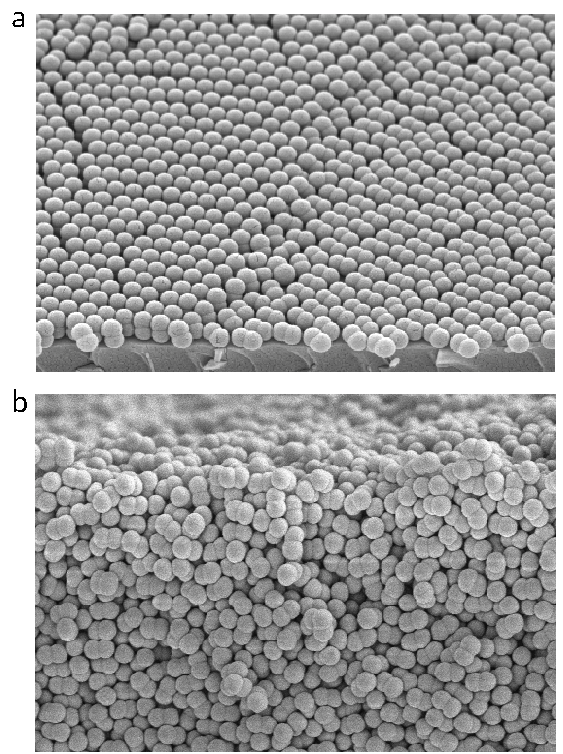
\includegraphics[width=0.9\textwidth]{figures/CFigure1.pdf}
\caption{\label{fig:assembly} \emph{Dumbbells crystallize in confinement, but not in the bulk.}
	\emph{a}), SEM image of dry dumbbells cast into thin films by vertical deposition. Dumbbells form ordered mono- and bi-layers \cite{Park2010}.
	\emph{b}), SEM image of dumbbells cast into an amorphous thick film. The fields of view in (a) and (b) are 7.6 $\mu$m across.}
\end{figure*}

While these dumbbells  readily crystallize in confined films \cite{Park2010}, they resist crystallization in the bulk.
As the film thickness increases, dumbbells form ordered monolayers laying down, ordered monolayers standing up, as shown in Figure~\ref{fig:assembly}a, and three variations of ordered bilayers (down/down, down/up and up/up) \cite{Park2010}.
However, when these dumbbells are dried into a film of even three layers, they pack randomly, as shown in Figure~\ref{fig:assembly}b.
These observations are at odds with numerical simulations predicting the equilibrium phase diagram of hard dumbbells, which suggests that these particles should form structures with long-range order in thermodynamic equilibrium at these volume fractions  \cite{Vega1992}.


\section{Electric-Field Assisted Crystallization}

To adopt a crystalline packing, dumbbells not only have to arrange themselves on a periodic lattice, but also have to orient themselves in a specific direction.
In order to facilitate crystallization, we bias the particle orientations with an external electric field \cite{Mittal2009, Grzelczak2010, Demirors2010}.
The anisotropic polarizability of dumbbells causes them to align themselves with the direction of the electric field.
The applied electric field also introduces long range interactions between particles which tend to locally concentrate the suspension \cite{Fraden1989, Yethiraj2003, Gong2003, Mittal2008}.
In Figure~\ref{fig:device}, we demonstrate the capability to control the structure  of dumbbell suspensions with an external electric  field.
With no applied electric field, the suspension is strongly scattering with no structural color or birefringence.
Initially, the sample is gray when viewed under crossed polarizers because the random orientations and positions of the dumbbells act to mix the polarization of light propagating through the sample.
We then apply an AC electric field ($f=50$ kHz, $E=$ 1040 V/cm) with co-planar gold electrodes separated by a 0.85 mm gap in a 20 $\mu$m thick glass sample chamber, a schematic of the chamber is shown in Figure~\ref{fig:schematic}.
The sample cell is placed between crossed polarizers, which are at an angle of approximately 45 degrees to the field direction.
Digital color movies are recorded on an inverted Axiovert 200 Zeiss microscope using a digital SLR camera (Canon-EOS Digital Rebel T1i).
About six seconds after the field is turned on we see a wave of birefringence originating from the electrodes, where the electric field strength is highest.
Within 36 seconds, there is strong birefringence and structural color visible throughout the bulk.
The patchwork of structural color across the sample points to polycrystalline domains on the order of 7 microns in width.
The crystallites can be further compacted by a step change in the frequency of the applied electric field (from 50 to 10 kHz), which can be seen in Supplementary Movie 2 of Ref.~\cite{Forster:2011}, which changes the form of the interparticle dipole interaction \cite{Mittal2008}.
When the electric field is turned off,  structural color and birefringence rapidly disappear.
We quantify the difference in on and off rate by plotting the ratio of the intensity in the red channel to the total intensity of Supplementary Movie 1 of Ref.~\cite{Forster:2011} in Figure~\ref{fig:movie-quantification}.
Field-switchable photonic crystals have previously been demonstrated with spherical particles \cite{Lumsdon2003}, but suspensions of dumbbells may offer more flexibility and speed.

\begin{figure*}[htbp]
\centering
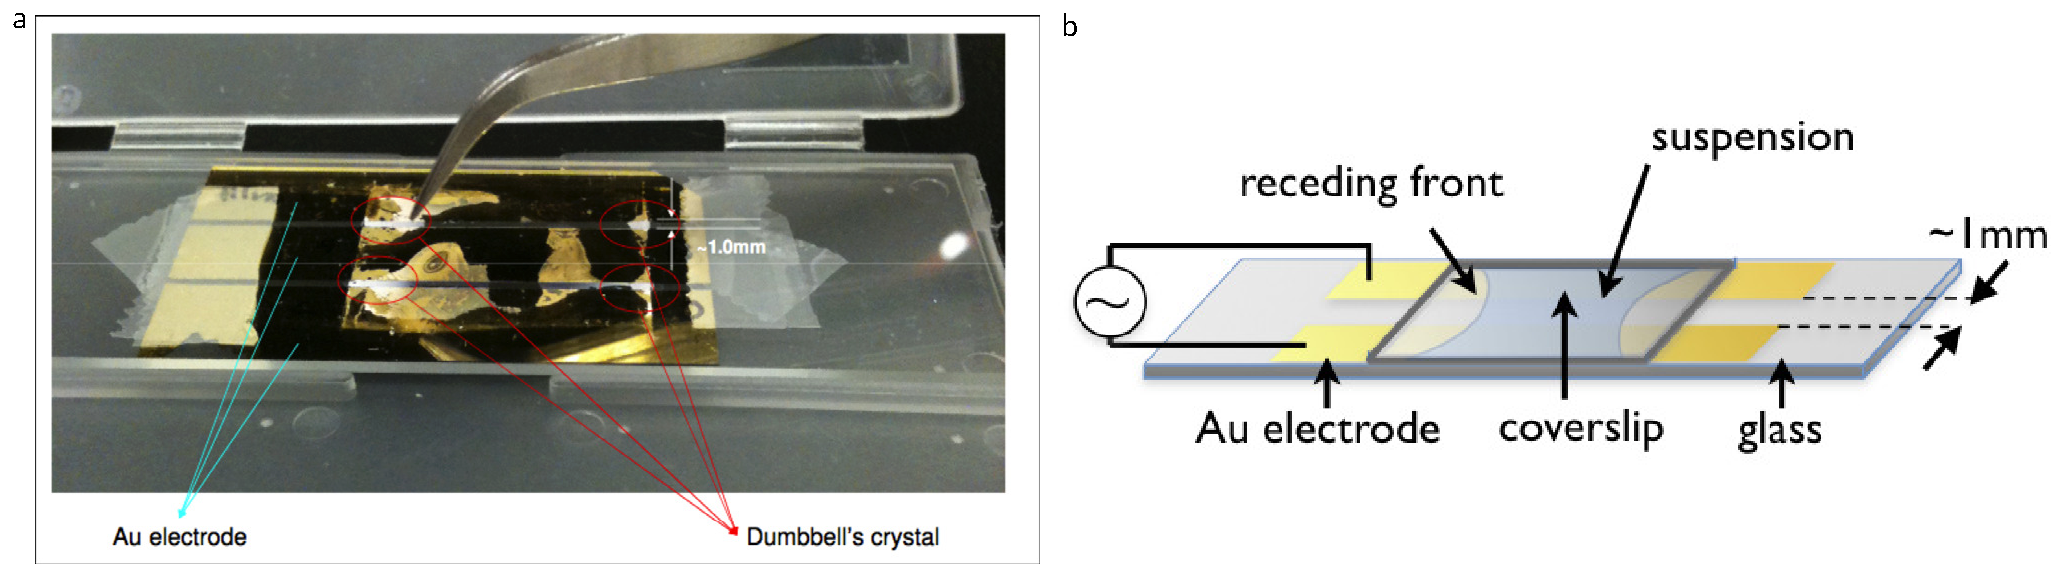
\includegraphics[width=1.0\textwidth]{figures/CsuppFigure1.pdf}
\caption{\label{fig:schematic} \emph{Sample chamber details.}
	\emph{a}), Photograph of the sample chamber used to make dumbbell crystals.
	\emph{b}), Schematic of the sample chamber.}
\end{figure*}

\begin{figure*}[htbp]
\centering
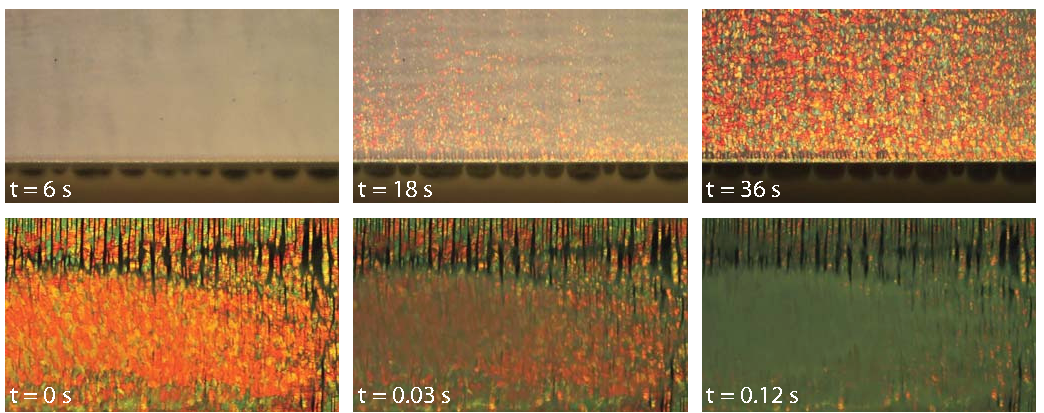
\includegraphics[width=1.0\textwidth]{figures/CFigure2.pdf}
\caption{\label{fig:device} \emph{Aqueous suspensions of dumbbells display reversible crystallization in AC electric fields.}
	Aqueous suspension of dumbbells at volume fraction  $\phi=$ 0.13.
  	\emph{Top row}, Snap shots showing the onset of crystallization in an aqueous suspension of dumbbells in an AC electric field. The dark stripe across the bottom of the frame is a gold electrode. The sample is imaged through crossed polarizers.
  	\emph{Bottom row}, Snap shots showing the rapid loss of structural color and birefringence when the electric field is turned off. The whole process can be seen in Supplementary Movie 1 of Ref.~\cite{Forster:2011}. The field of view in each image is 1.4 mm across.}
\end{figure*}

\begin{figure*}[htbp]
\centering
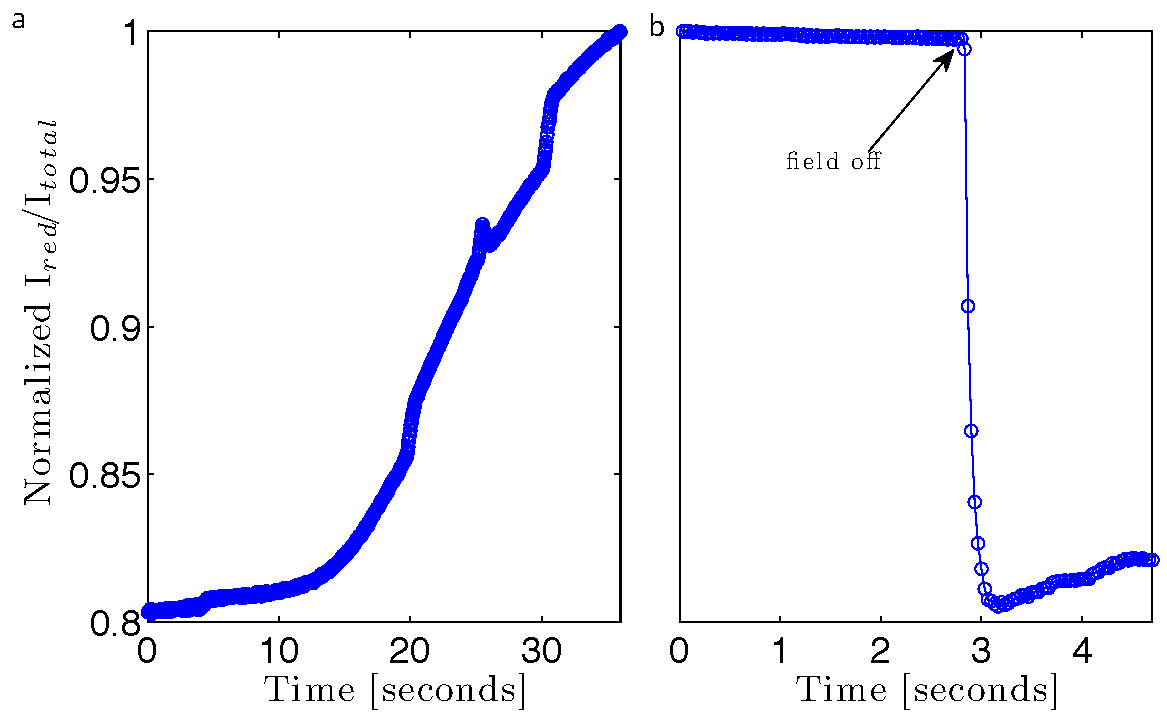
\includegraphics[width=1.0\textwidth]{figures/CsuppFigure2.pdf}
\caption{\label{fig:movie-quantification} \emph{The timescales for the onset and disappearance of structural color and birefringence are very different.}
	Ratio of the intensity in the red channel to the total intensity from the video of \emph{a}) crystal formation and \emph{b}) crystal melting.}
\end{figure*}

 To assemble stable crystalline packings, we dry dumbbell suspensions  in the presence of an electric field.
 The crystal seen in  Figure~\ref{fig:structure1}a is approximately one hundred particles thick, and is the result of the application of an AC electric field ($f=50$ kHz, $E=$ 1040 V/cm) during the unidirectional drying of an aqueous suspension of dumbbells with initial volume fraction, $\phi=$ 0.13 \cite{Mittal2009}.
 Additional SEM images of the resulting structures can be seen in Figure~\ref{fig:crystalSEM1} - \ref{fig:crystalSEM4}.
 Previous studies have used magnetic fields to align ellipsoidal particles during convective assembly but were only able to achieve crystal thicknesses of approximately 20 particle layers \cite{Ding2009}.

\begin{figure*}[htbp]
\centering
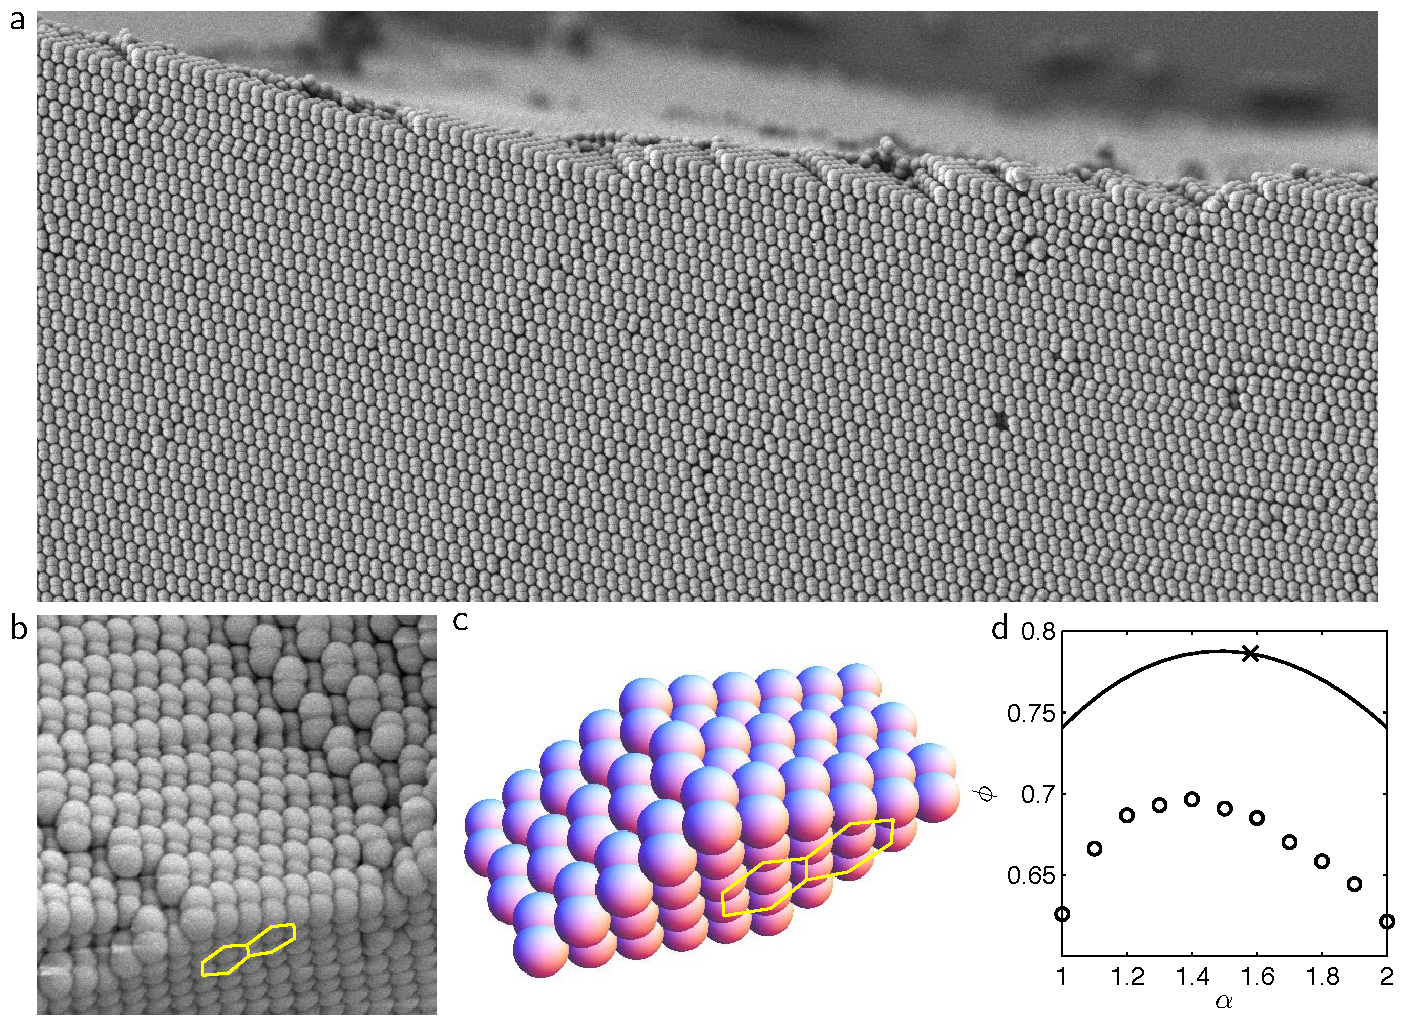
\includegraphics[width=1.0\textwidth]{figures/CFigure3.pdf}
\caption{\label{fig:structure1} \emph{Crystal structure of suspension dried in an AC electric field.}
	\emph{a}), SEM image of crystal formed by drying a suspension of dumbbells in the presence of an electric field. In this image, the electric field orientation is approximately vertical and the direction of flow due to drying is from right to left. The field of view is 27 $\mu$m across.
	\emph{b}), SEM image highlighting crystal structure. Two adjoining hexagons formed by the dumbbell lobes are highlighted by the yellow hexagons. The field of view is 3.6 $\mu$m across.
	\emph{c}), Model of the crystal structure suggested by SEM images. Two adjoining hexagons are highlighted and correspond to the highlighted facet in (b).
	\emph{d}), Packing fraction versus aspect ratio for crystalline structures (line) and random, jammed packings (circles) generated from numerical simulations described in the methods section. The packing fraction for the aspect ratio 1.58 dumbbells in a crystalline structure is $\phi = 0.7862$ (x).}
\end{figure*}

\begin{figure*}[htbp]
\centering
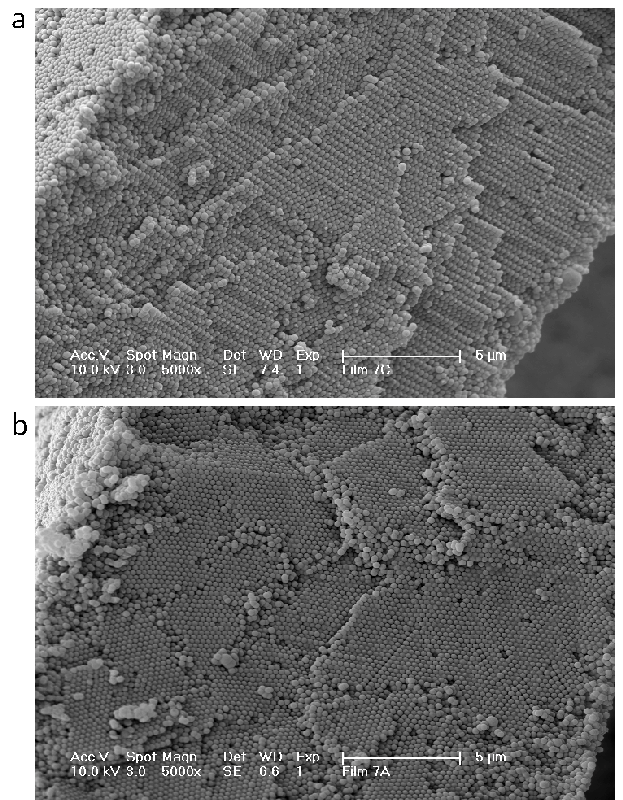
\includegraphics[width=1.0\textwidth]{figures/CsuppFigure3.pdf}
\caption{\label{fig:crystalSEM1} \emph{SEM images showing different cross-sectional views of a dumbbell crystal.}
	\emph{a}), The electric field direction relative to this image is approximately from bottom left to top right.
	\emph{b}), The electric field direction relative to this image is approximately into the page.}
\end{figure*}

\begin{figure*}[htbp]
\centering
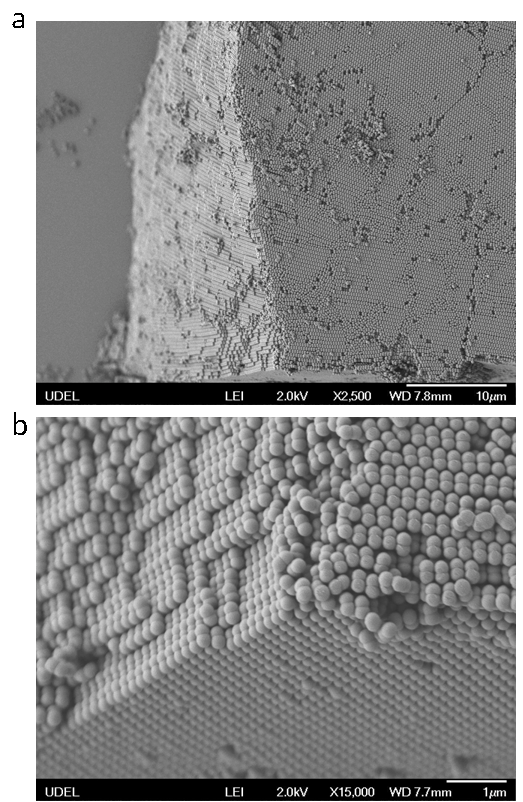
\includegraphics[width=0.8\textwidth]{figures/CsuppFigure4.pdf}
\caption{\label{fig:crystalSEM2} \emph{SEM images showing details of a dumbbell crystal.}
	\emph{a}), The electric field direction relative to this image is approximately vertical.
	\emph{b}), The electric field direction relative to this image is approximately vertical.}
\end{figure*}

\begin{figure*}[htbp]
\centering
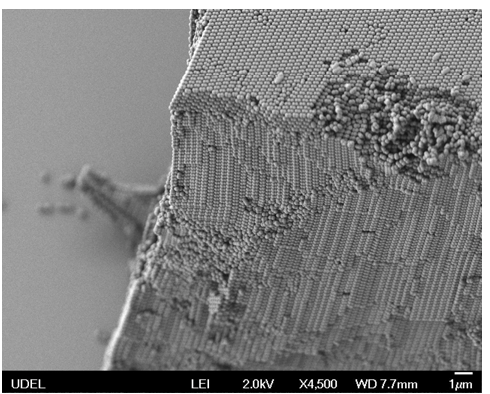
\includegraphics[width=1.0\textwidth]{figures/CsuppFigure5.pdf}
\caption{\label{fig:crystalSEM3} \emph{SEM image of a dumbbell crystal.}
	The electric field direction relative to this image is approximately horizontal.}
\end{figure*}

\begin{figure*}[htbp]
\centering
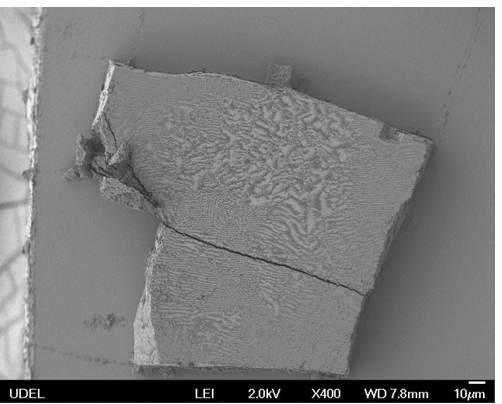
\includegraphics[width=1.0\textwidth]{figures/CsuppFigure6.pdf}
\caption{\label{fig:crystalSEM4} \emph{SEM image of a dumbbell crystal.}
	Low magnification SEM image of a dumbbell crystal. The Moire fringes in the image indicate that there is long-range order in the sample.}
\end{figure*}


\section{Structural Properties of Dumbbell Crystals}

 The crystal structure formed by dumbbells is more complicated than the cubic structures formed by spherical particles.
 SEM images of the dumbbell crystals reveal a number of features that allow us to identify the structure.
 In the bottom of Figure~\ref{fig:structure1}b one can see lobes of the dumbbells in hexagonally-packed layers, highlighted by yellow hexagons, with the major axis of the dumbbells tilted relative to the normal of these planes.
 Successive layers pack such that the hexagonally-packed bottom lobes of a new layer fit into the hexagonally-packed top lobes of the previous layer.
 This layering scheme allows for successive layers to fit snugly together for any particle tilt, so long as the top and bottom lobes of each particle can remain in contact with the top and bottom lobes of its six nearest neighbors.
 For ordered close-packed spheres, there are three possible translational alignments of one hexagonally packed layer with respect to the next, which specify the familiar FCC, HCP and RHCP packings.
 Dumbbells have an additional three-fold orientational degeneracy, due to the tilting of the particles within each layer.
 However, in an applied electric field, the dumbbells tend to maintain a constant orientation from plane to plane, as shown in Figure~\ref{fig:structure1}a,b.
 A schematic of this packing is shown in Figure~\ref{fig:structure1}c.
During drying, capillary forces tend to drive suspended particles toward their densest packing.
 To our knowledge, this packing, which was found to be equilibrium structure of hard dumbbells \cite{Vega1992} is the densest packing of symmetric dumbbells.
 In numerical simulations, we have verified that this packing is mechanically stable and at least a local maximum in the packing density, as described in Figure~\ref{fig:mechanical-stability}.

\begin{figure*}[htbp]
\centering
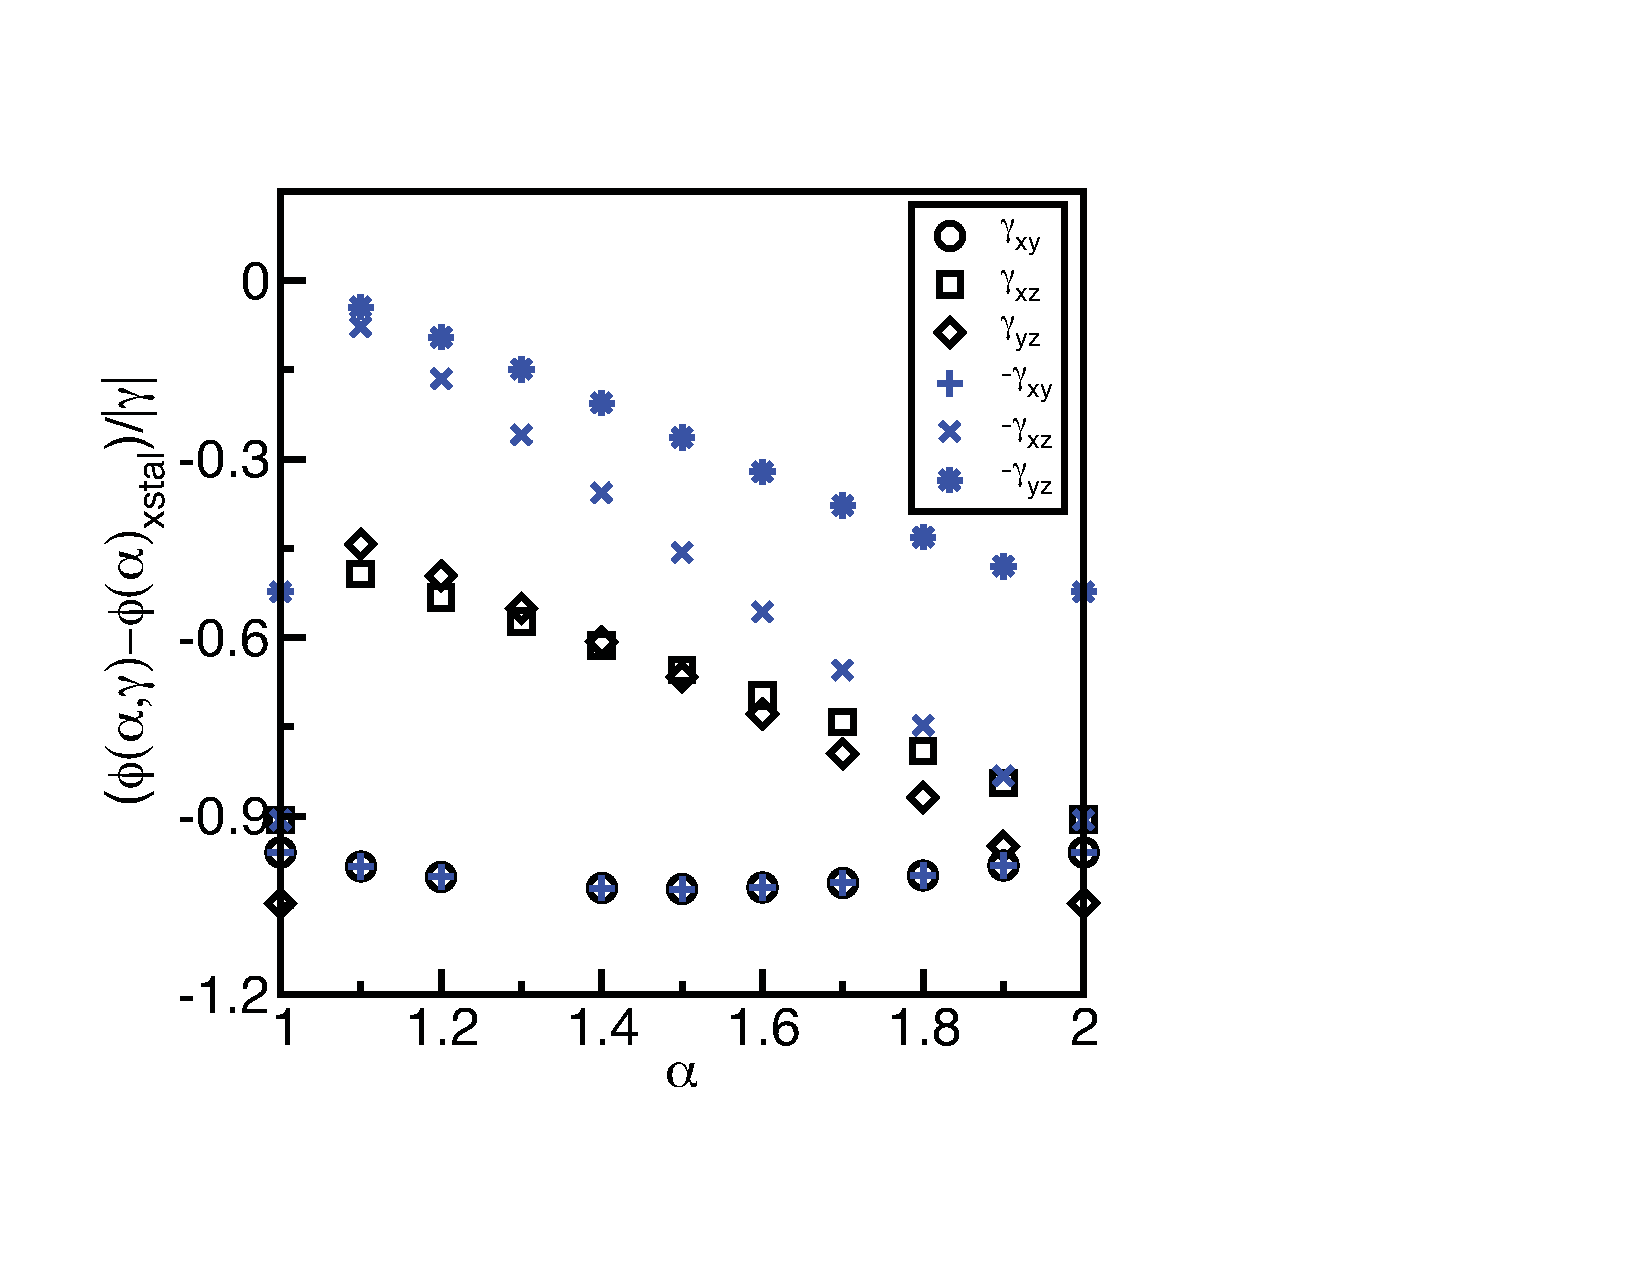
\includegraphics[width=1.0\textwidth]{figures/CsuppFigure7.pdf}
\caption{\label{fig:mechanical-stability} \emph{The crystalline dumbbell structure described here is at least the densest local structure with respect to all possible linear strains of the cubic boundary.}
	To show this, we first create a mechanically stable crystalline packing by initializing the system with crystal positions and orientations and then apply the isotropic compression protocol to relax it. We obtain packing fractions $\phi_J \approx \phi_{xstal} + 10^{-8}$, which is consistent with the fact that the stopping criterion allows infinitesimal overlaps with $V/N\epsilon\approx 10^{-16}$. We then perturb the box shape using three orthogonal infinitesimal strains $\gamma_{xy}$, $\gamma_{xz}$, and $\gamma_{yz}$ in both the positive and negative strain directions, and use the isotropic compression protocol at fixed strain to find the nearest mechanically stable packing with $\phi_J(\gamma)$. The packing fraction decreases, $\phi_{xstal}-\phi_J(\gamma)<0$ for all aspect ratios and perturbations we studied.}
\end{figure*}

 These structures have very high packing fractions.
 For the dumbbells used in our experiments, the  packing fraction is $\phi=$ 0.7862.
 This packing fraction is significantly higher than both the densest crystalline sphere packing, $\phi^{FCC}_{sphere}=$ 0.7405, and the densest known crystalline packing of ellipsoids, $\phi_{ellipsoid}=$ 0.7707 \cite{Donev2004}.
  Figure~\ref{fig:structure1}d shows the anticipated packing fraction of dumbbells in this crystal structure as a function of aspect ratio, 
\begin{equation}\label{eqn:phi-vs-aspect}
\phi = \frac{(3-\alpha)\alpha^2}{2+(\alpha-1)\sqrt{6-2(\alpha-1)^2}}\phi^{FCC}_{sphere}.
\end{equation}
 The aspect ratio that gives the highest packing fraction is 1.5, with $\phi=$ 0.7877.
 The dumbbell tilt angle for the crystal structure depends on aspect ratio, as shown in Figure~\ref{fig:tilt-angle}.
 For aspect ratios 1.5 and 1.58, the tilt angles for the crystal structure are 16.8 and 19.5 degrees, respectively.

\begin{figure*}[htbp]
\centering
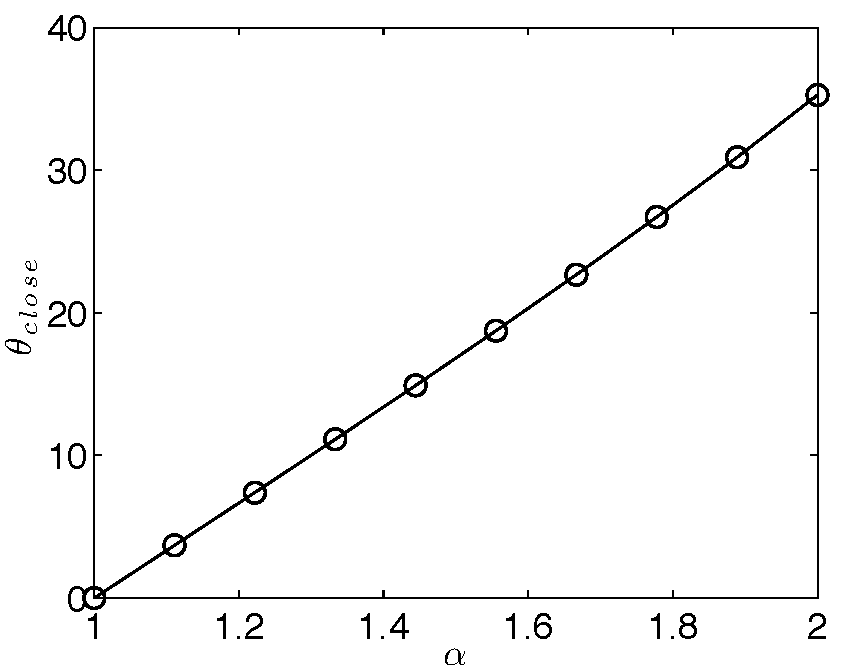
\includegraphics[width=1.0\textwidth]{figures/CsuppFigure8.pdf}
\caption{\label{fig:tilt-angle}
  	Angle of dumbbell tilt that corresponds to the maximum packing fraction as a function of dumbbell aspect ratio, $\alpha$.}
\end{figure*}

 Our experiments suggest that restricting the orientation of the dumbbells is critical to achieving crystallization -- numerical simulations of the jamming of dumbbells under compression yield similar findings.
 We perform numerical simulations of mechanically stable dumbbell packings by successively compressing and decompressing the system and relaxing the energy until all forces are balanced and inter-particle overlaps are vanishingly small \cite{Gao2006}.
 The probability of the system crystallizing as a function of aspect ratio $\alpha$ for slow thermal quench rates is plotted in Figure~\ref{fig:structure2}.
 In the absence of an external field that favors alignment, systems of dumbbells with $\alpha$ higher than 1.1 have essentially zero probability of crystallizing at the quench rates explored here.
  By contrast, restricting particle orientations dramatically increases the probability of crystallization.
 In that case, the probability of crystallization is highest for aspect ratios between 1.2 and 1.6.
 Previous Monte Carlo simulations predict that the crystalline phase we observe should be thermodynamically stable for $\alpha$ greater than 1.3 even in the absence of an external field \cite{Vega1992b}.
 However, in our simulations in the absence of the field, the particles form amorphous mechanically stable packings at densities that are systematically lower than their crystalline counterparts as plotted in Figure~\ref{fig:structure1}d, and also lower than random jammed packings of oblate ellipsoids \cite{Donev2004, Donev2004b}.
 We find that lowering the quench rate used in our simulations by a factor of 1000 does not have a significant effect on the probability of crystallization for either the aligned or unrestricted dumbbells, as seen in Figure~\ref{fig:structure2}.
  We perform extensive numerical simulations of soft dumbbell particles composed of two rigidly-constrained spheres.
 The interactions between dumbbell particles arise from purely repulsive, pairwise linear spring forces that act centrally between the centers of the spheres that comprise two different dumbbells.
 We generate mechanically stable dumbbell packings via isotropic compression---by successively compressing and decompressing the system and relaxing the energy until all forces and torques are balanced and inter-particle overlaps are vanishingly small using the algorithm described in detail in \cite{Gao2006}.
 To create the amorphous mechanically stable dumbbell packings described in Figure~\ref{fig:structure1}d, we initialize the system in a dilute state at packing fraction $\phi_0=0.2$ with random dumbbell positions and orientations inside a unit cube.
 We  choose the increment in packing fraction as $\Delta\phi\leq 10^{-4}$ and the final potential energy $V/\epsilon N$ of the packing to be in the range $10^{-16} < V/\epsilon N < 2\times 10^{-16}$, where $\epsilon$ is the characteristic energy scale of the repulsive interaction and $N=512$ is the number of dumbbells.
 We also perform simulations to compare the probability to form a crystalline structure in the presence and absence of a strong aligning field as shown in Figure~\ref{fig:structure2} in systems ranging from $N=27$ to $125$ particles.
 We thermally quench equilibrated fluid systems at $\phi_0 =\phi_{xstal}-0.2$ and $k_b T/\epsilon = 10^{-3}$ by linearly decreasing the temperature to $T = 0$ over a wide range of thermal quench rates $10^{-2} > r k_b T \tau/\epsilon > 10^{-9}$ to generate the initial configurations, where $\tau$ is a typical collision time between dumbbells.
 In Figure~\ref{fig:structure2}, we show results for $r k_b T \tau/\epsilon =10^{-6}$ and $r k_b T \tau/\epsilon =10^{-9}$ since these rates yield FCC packings for spheres.
 We then use the isotropic compression protocol described above with initial configurations from the thermal quenches to generate dumbbell packings.
 To simulate a strong aligning field, the orientations are initially chosen to be consistent with the crystalline packing at each aspect ratio, and then prevented from evolving during the thermal quench and isotropic compression packing algorithm.
 The fraction of crystalline packings $P_{xtal}$ is determined as the ratio of the number of packings with $|\phi_{xstal}-\phi_J| < 10^{-6}$ to the total number of trials.
 
\begin{figure*}[htbp]
\centering
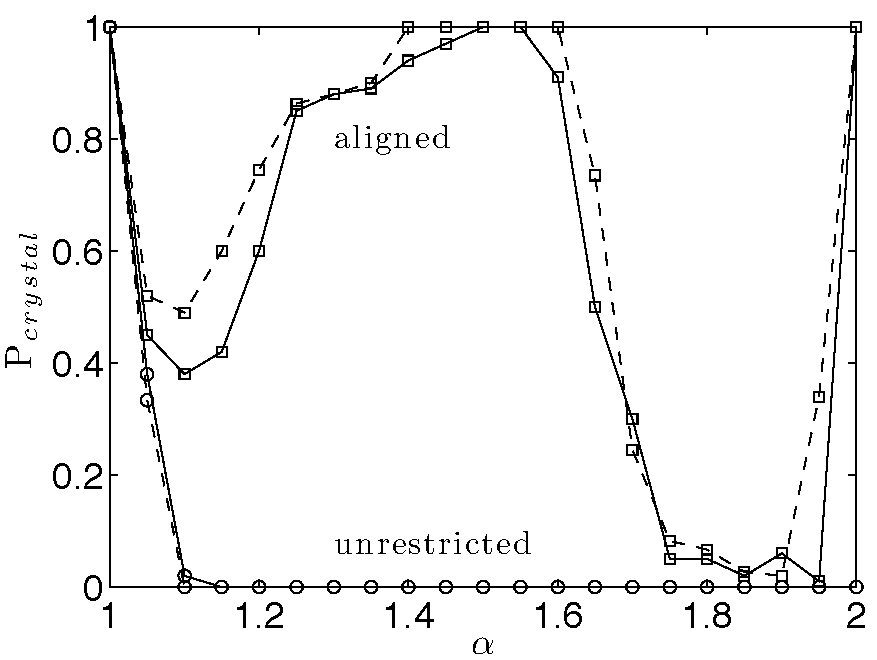
\includegraphics[width=1.0\textwidth]{figures/CFigure4.pdf}
\caption{\label{fig:structure2} \emph{Simulations demonstrate crystal formation depends strongly upon control of dumbbell orientation.}
	Probability of crystallization for a system of dumbbells as a function of aspect ratio. Systems with aligned dumbbells (squares) have significant probabilities of crystallization for most aspect ratios. Systems with unrestricted dumbbell orientations (circles) have near zero probabilities of crystallization for aspect ratios greater than  1.1. Each point is the result of 100 independent simulations. The two line types represent simulations performed with different quench rates, the dashed line has a quench rate that is 1000 times lower than the solid line.}
\end{figure*}


\section{Photonic Properties of Dumbbell Crystals}

These dumbbell crystals have partial photonic band gaps.
Figure~\ref{fig:optics}a shows a normal incidence reflection spectrum of a 70 $\mu$m x 70 $\mu$m area of a dumbbell crystal measured with a Nikon Optiphot 66 Microscope in epi-scopic mode.
We use a 40X objective lens for illumination and collection of reflected light, and use a field stop to reduce the size of the illumination and collection area.
The reflected light is transferred to an Ocean optics HR2000+ spectrometer through an optical fiber and normalized to the spectrum recorded from an Ocean Optics reflection standard.
We see a strong peak in the reflectance at 644 nm with a full width at half maximum (FWHM) of 72 nm.
Using our model of the crystal structure, we calculate the photonic band structure.
These calculations show partial band gaps in certain crystal directions, as described in Figure~\ref{fig:band-structure}.
In the direction optical reflection was probed (Figure~\ref{fig:optics}a), the predicted photonic band gap is centered at 660 nm with a FWHM of 30 nm.
The center wavelength matches well that of the reflection peak in Figure~\ref{fig:optics}a, but the width is significantly smaller.
We believe the presence of multiple domains with different crystal orientations, as seen in the SEM images, leads to a spectral broadening of the reflectance peak.

\begin{figure*}[htbp]
\centering
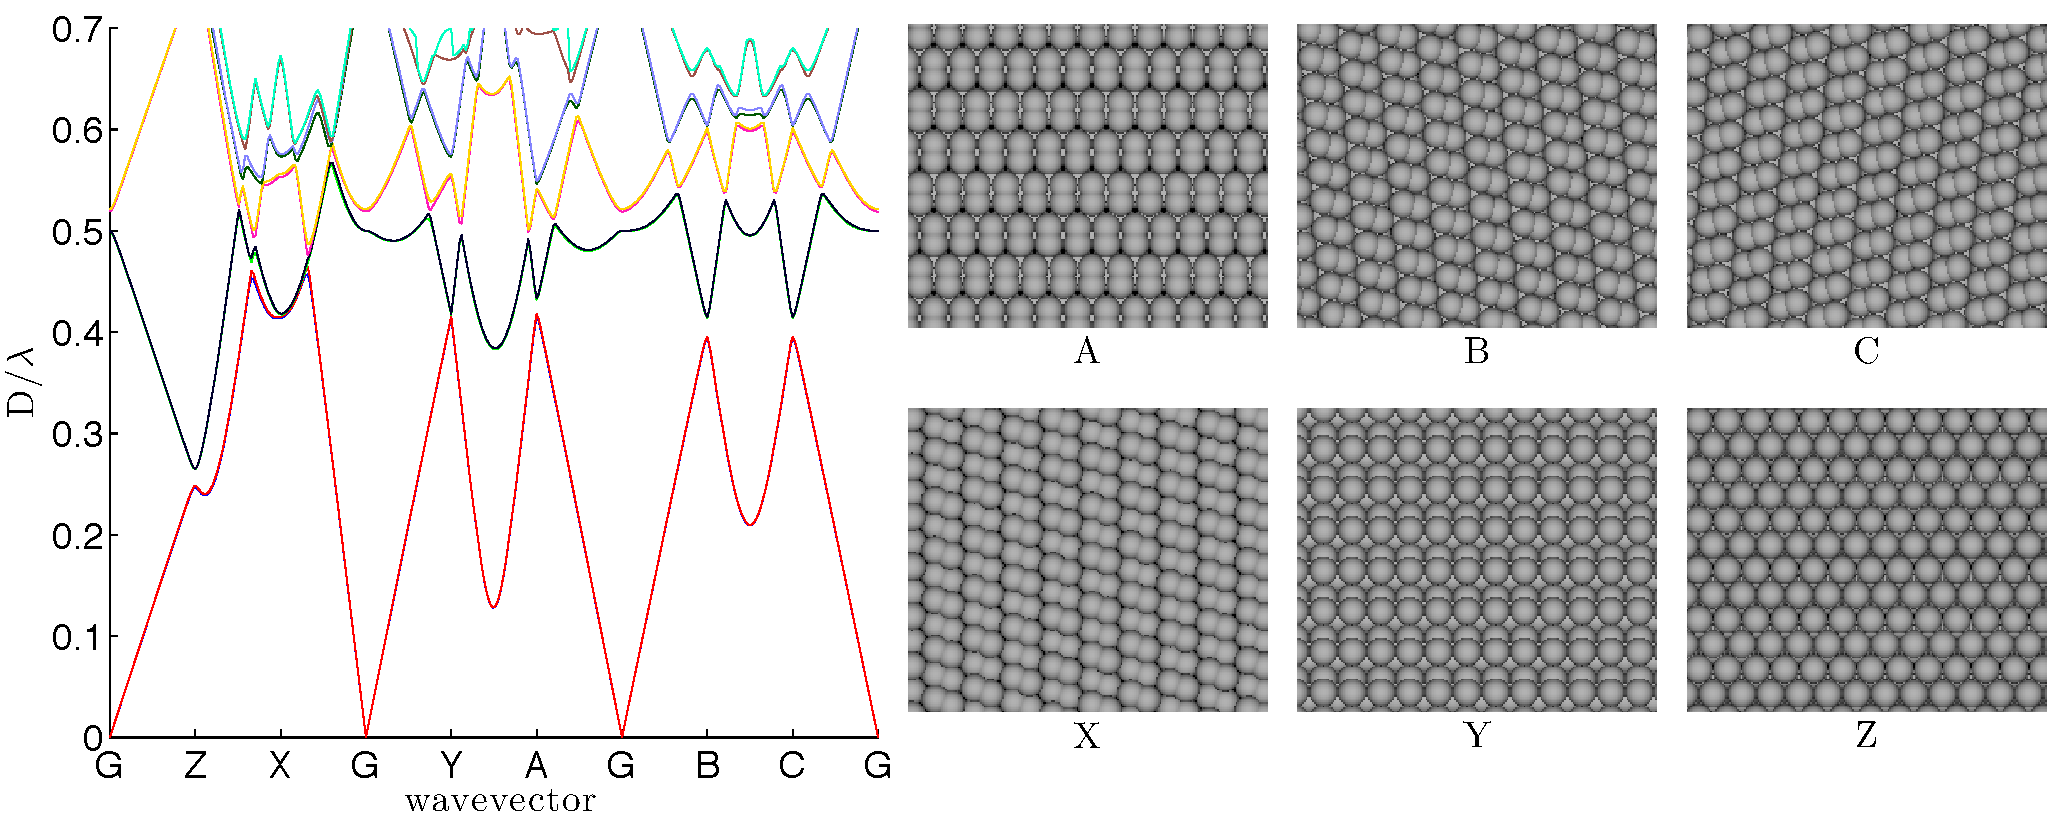
\includegraphics[width=1.0\textwidth]{figures/CsuppFigure9.pdf}
\caption{\label{fig:band-structure}\emph{Photonic band structure.}
  	\emph{Left panel:} Photonic band structure, where D is the diameter of one dumbbell lobe, 267 nm for the dumbbells we use.
	\emph{Right panel:} Illustrations corresponding to the crystal orientations for each wave vector.}
\end{figure*}

In addition to having a photonic band gap, these dumbbell crystals are birefringent.
To visualize the birefringence, we image the crystals through crossed polarizers using wavelengths inside and outside the band gap (650 and 534 nm).
For both wavelengths, we observe a sinusoidal modulation of the transmitted intensity with the relative angle of the sample and crossed polarizers, as seen in Supplementary Movies 3 (650 nm) and 4 (534 nm) of Ref.~\cite{Forster:2011}.
The depth and phase of the modulation varies from location to location within the sample, as shown in Figure~\ref{fig:optics}b,c and Figure~\ref{fig:optics2}.
Depolarization of transmitted light inside the band gap is expected from the previous studies of colloidal crystals due to the polarization-dependent efficiency of Bragg diffraction from the crystal structure \cite{Monovoukas1990}.
In contrast, we also observe strong birefringence outside of the photonic band gap, where crystals of colloidal spheres would not be birefringent.
Since this light is not diffracted by the crystal's Bragg planes, we believe that the birefringence originates from the anisotropic shape of individual dumbbell particles.
The images of transmitted intensity during the rotation of crossed polarizers in Figures~\ref{fig:optics}b,c and ~\ref{fig:optics2} are recorded on a Nikon TE-2000 inverted optical microscope with a Photron FASTCAM 1024 PCI camera. 
The halogen bright field lamp on the microscope is used for illumination and colored filters are used to select wavelengths inside and outside the photonic band gap.
 
\begin{figure*}[htbp]
\centering
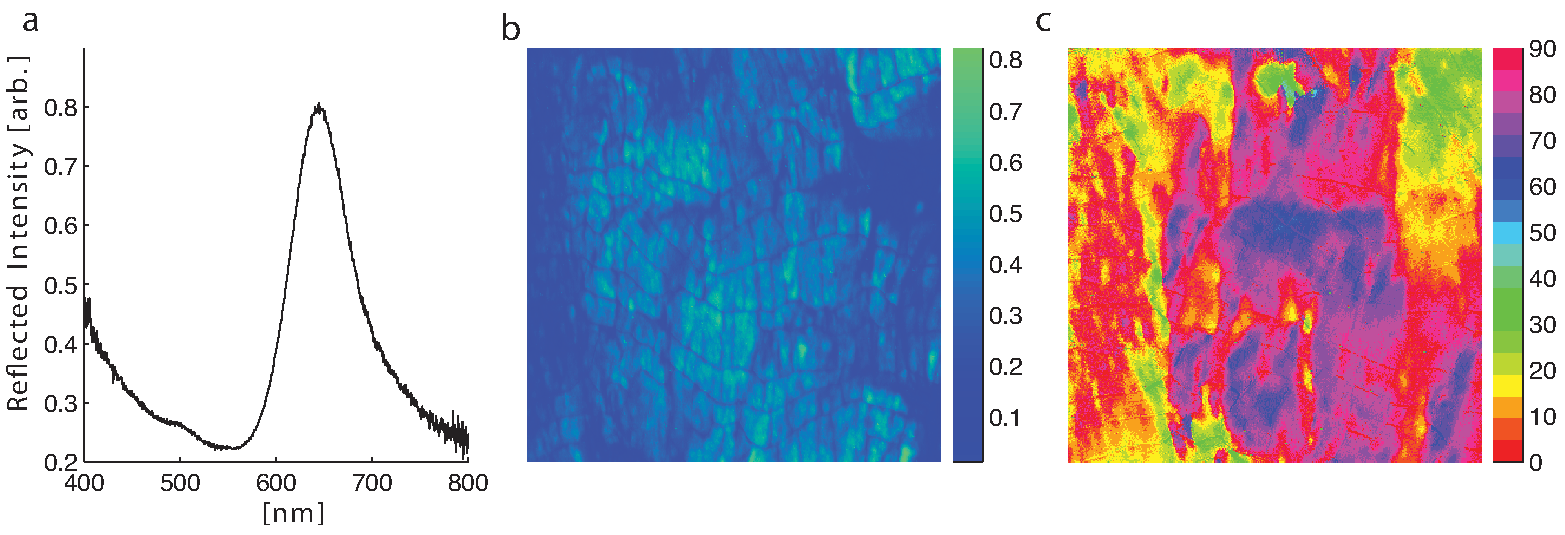
\includegraphics[width=1.0\textwidth]{figures/CFigure5.pdf}
\caption{\label{fig:optics} \emph{Dumbbell crystals have a partial photonic band gap and are birefringent.}
	\emph{a}), Normal incidence reflection spectrum from a 70 $\mu$m x 70 $\mu$m area of a dumbbell crystal. The peak at 644 nm is close to the predicted photonic band gap position for the probed direction (band diagram in Figure~\ref{fig:band-structure}). 
	Images of \emph{b}) the depth and \emph{c}) phase of the modulation (in degrees) of transmitted light with the rotation of crossed polarizers measured at a wavelength of 650nm, which is inside the band gap. The electric field direction relative to this image is vertical. The field of view in both (b) and (c) is 600 $\mu$m across.}
\end{figure*} 
 
\begin{figure*}[htbp]
\centering
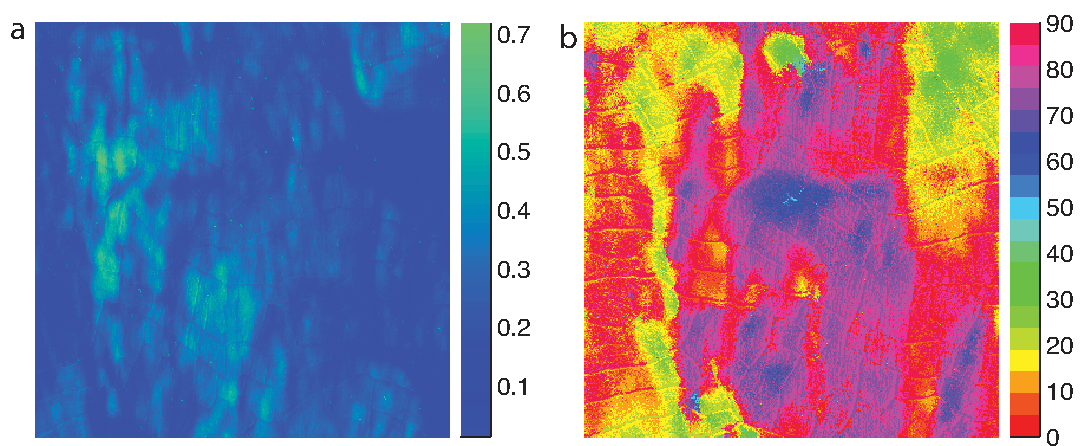
\includegraphics[width=1.0\textwidth]{figures/CsuppFigure10.pdf}
\caption{\label{fig:optics2}
  	Images of \emph{a}) the depth and \emph{b}) phase of the modulation (in degrees) of transmitted light with the rotation of crossed polarizers measured at a wavelength of 534 nm, which is outside the band gap. 	The electric field direction relative to this image is vertical. The field of view in both (a) and (b) is 600 $\mu$m across.}
\end{figure*} 

Anisotropic colloidal particles can self assemble into crystalline structures with long-range order in the presence of an external field.
Crystals of anisotropic particles have novel optical properties which combine photonic band gaps with birefringence.
Furthermore, anisotropic particles could improve the speed and functionality of field-switchable photonic crystals by allowing dramatic changes to optical properties through mere particle reorientation and not complete reorganization of the underlying suspension structure.

